\documentclass[10pt]{report}
\usepackage[utf8]{inputenc}
\usepackage[T1]{fontenc}
\usepackage[english]{babel}
\usepackage{fourier} % Nicenesss font
\usepackage{amsfonts,amsmath}
\usepackage[pdftex]{color,graphicx}
\usepackage{pdfpages}
\usepackage{fancyhdr}
\usepackage{textcomp}
\usepackage{lmodern}
\usepackage{xcolor}
\usepackage{multicol}
\usepackage{soul}
\usepackage{algorithmic}
\usepackage{wrapfig}
\usepackage{float}
\usepackage{mdwlist}
\usepackage{pgfgantt}
\usepackage{a4wide}
\usepackage{tabularx}
\usepackage{booktabs}

\newcommand{\tabitem}{~~\llap{\textbullet}~~}

\usepackage{hyperref}
\usepackage{lscape}

\usepackage{sectsty}
\allsectionsfont{\centering \normalfont\scshape}
\renewcommand{\thesection}{\arabic{section}}

\numberwithin{equation}{section} % Number equations within sections (i.e. 1.1, 1.2, 2.1, 2.2 instead of 1, 2, 3, 4)
\numberwithin{figure}{section} % Number figures within sections (i.e. 1.1, 1.2, 2.1, 2.2 instead of 1, 2, 3, 4)
\numberwithin{table}{section} % Number tables within sections (i.e. 1.1, 1.2, 2.1, 2.2 instead of 1, 2, 3, 4)

%\usepackage{hyperref}
\pagestyle{fancy}
\newcommand{\HRule}{\rule{\linewidth}{0.5mm}}

%If in need of a header for the document, uncomment this and add desired text!
%\fancyhead[LO,LE]{}
%\fancyhead[RO,RE]{}
%

%Macro foo
\newcommand{\method}[3]{ \label{method:#2}
    {\vspace{10pt} \noindent \textbf{#1} \textit{#2}(#3)} :
}
\newcommand{\argument}[2]{{\textbf{#1} #2}}


%%%%%%%%%%%% END OF PREAMBLE %%%%%%%%%%%%%%%%%%%%%%%%%%%%%%%%%%%%
\begin{document}
\begin{titlepage}

\begin{center}

\textsc{\LARGE BDSA}\\[1.5cm]

\textsc{\Large System Design Document}\\[0.5cm]

\HRule \\[0.4cm]

{ \bfseries SDD \\[0.5cm] 
    {\small \today}} \\[0.7cm]

\HRule \\ [6.5cm]

% Author and supervisor
\begin{minipage}{0.5\textwidth}
\begin{flushleft} \large
Ahmed Al Aqtash (ahaq)\\
\textit{ahmed.aqtash@gmail.com}\\
Mikkel Åxman (mikx)\\
\textit{mikx@itu.dk}\\
Phillip Phoelich (ppho)\\
\textit{ppho@itu.dk}\\

\vfill 
\end{flushleft}
\end{minipage}
% Bottom of the page front page

\end{center}

\end{titlepage}
\clearpage
\begin{table}[h]
\begin{tabularx}{\textwidth}{l l X l}
\textbf{Version} & \textbf{Date} & \textbf{Description} & \textbf{Authors} \\ \midrule
1.0     & 9/9-2014 & First version of the SDD & ahaq, mikx, ppho \\
1.1     & 16/10-2014 & Added subsystem service diagram & ahaq\\
1.2     & 21/10-2014 & Added design pattern diagrams & ahaq, ppho\\
\end{tabularx}
\end{table}

\clearpage
%% Generelle struktur %%
\section{Introduction}
This is a breakdown of a simple calendar system, which provides means to
synchronise across multiple clients.

\subsection{Purpose of the system}
The purpose of this system is to provide users with a calendar system they can
use on any PC. In its current form, users can add calendars and events, and
synchronise these to a central server. Users should also be able to share
calendars.

\subsection{Design goals}
\subsubsection{Usability}
\begin{itemize}
\item A User must be able to successfully add a calendar in less than 30
  seconds, typing excluded.
\item A User must be able to add an event in less than 60 seconds, typing
  excluded.
\item A User must be able to add a calendar and publish it in less than 60
  seconds, bandwidth and typing excluded.
\end{itemize}
\subsubsection{Response time}
\begin{itemize}
\item Syncronising a calendar with the server should happen within 5 second,
  excluding differences in internet speeds.
\end{itemize}
\subsubsection{Fault tolerance}
\begin{itemize}
\item If the internet connection is lost, the User must be able to continue
  working. Changes will be syncronised with online calendar on reconnection.
\end{itemize}
\subsubsection{Robustness}
\begin{itemize}
\item An average user cannot give wrong input.
\end{itemize}
\subsubsection{Portability}
\begin{itemize}
\item The system should be able to be accessed from any given platform, running C\#.
\end{itemize}
\subsubsection{Extensibility}
\begin{itemize}
\item The way of storing calendars should be easily exchangeable.
\end{itemize}
%\subsubsection{Reliability}
%\subsubsection{Performance}
%\subsubsection{Supportability}
%\subsubsection{Implementation}
%\subsubsection{Interface}
%\subsubsection{Packaging}
%\subsubsection{Legal}
%\subsection{Definitions, acronyms, and abbreviations}
%\subsection{References}
%\subsection{Overview}
%
%\section{Current software architecture}
%
\section{Proposed software architecture}
%\subsection{Overview}

\subsection{Subsystem decomposition}
\begin{figure}[H]
  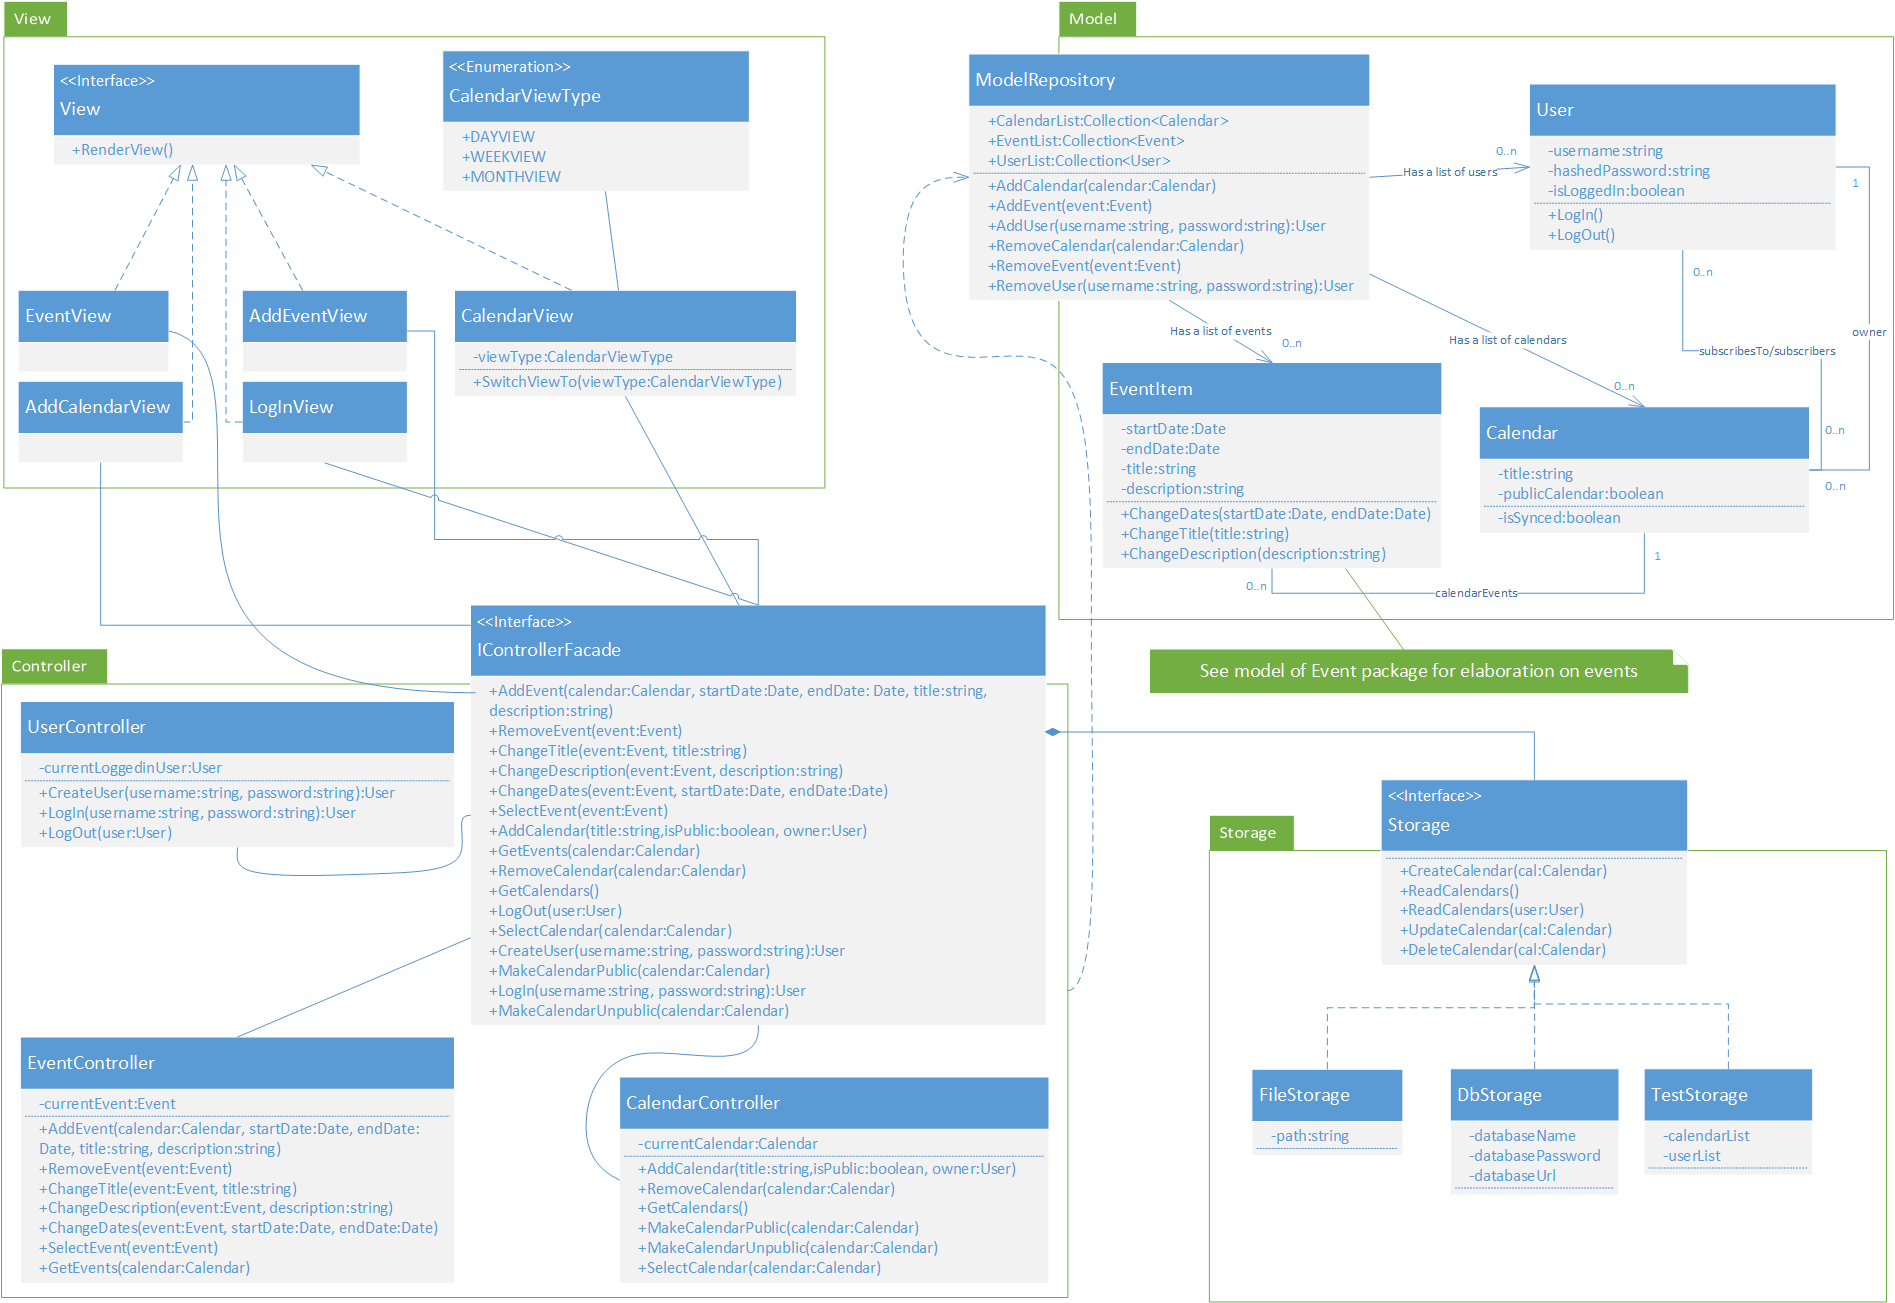
\includegraphics[scale=0.40]{figures/classdiagram.png}
\end{figure}

\begin{figure}[H]
  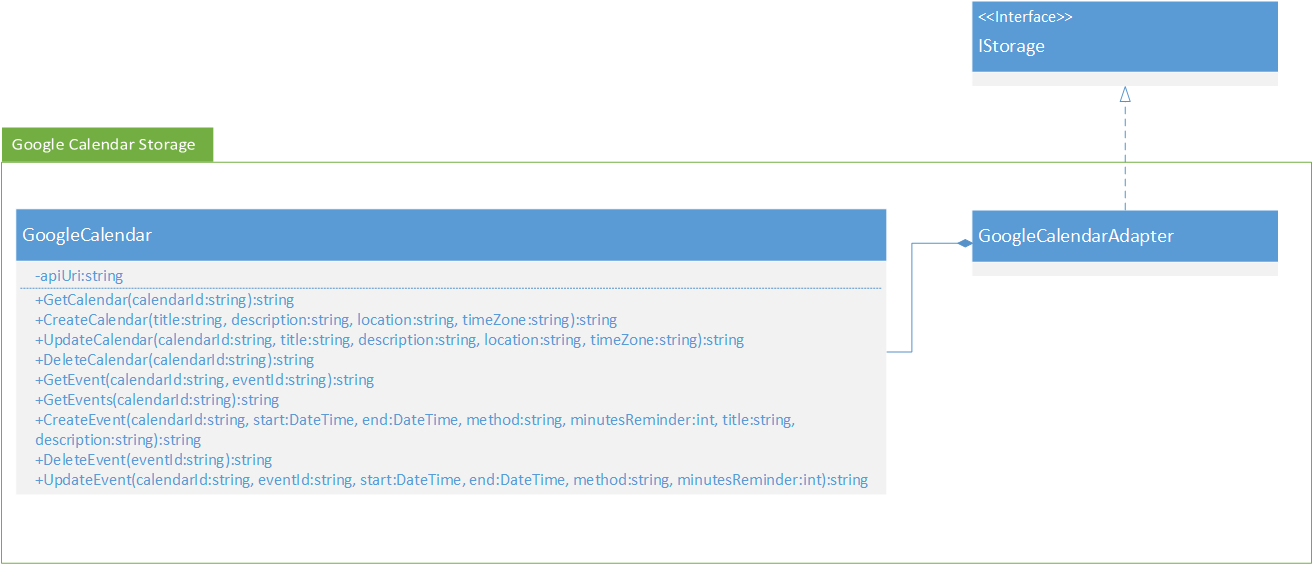
\includegraphics[scale=0.6]{figures/google_adapter.png}
\end{figure}

\begin{figure}[H]
  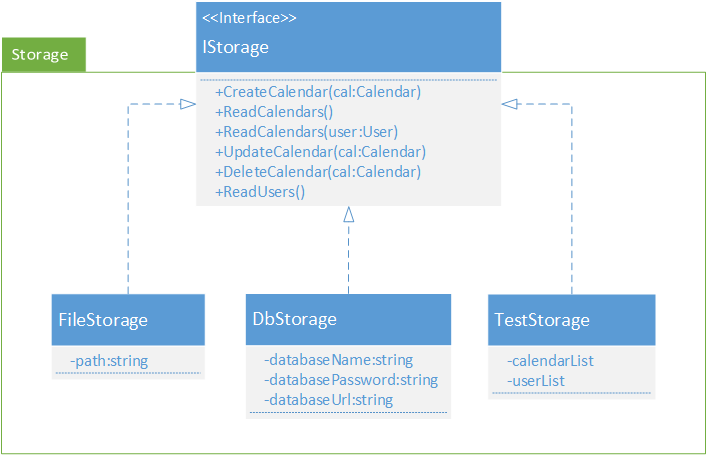
\includegraphics[scale=0.6]{figures/class_storage_bridge.png}
\end{figure}

\begin{figure}[H]
  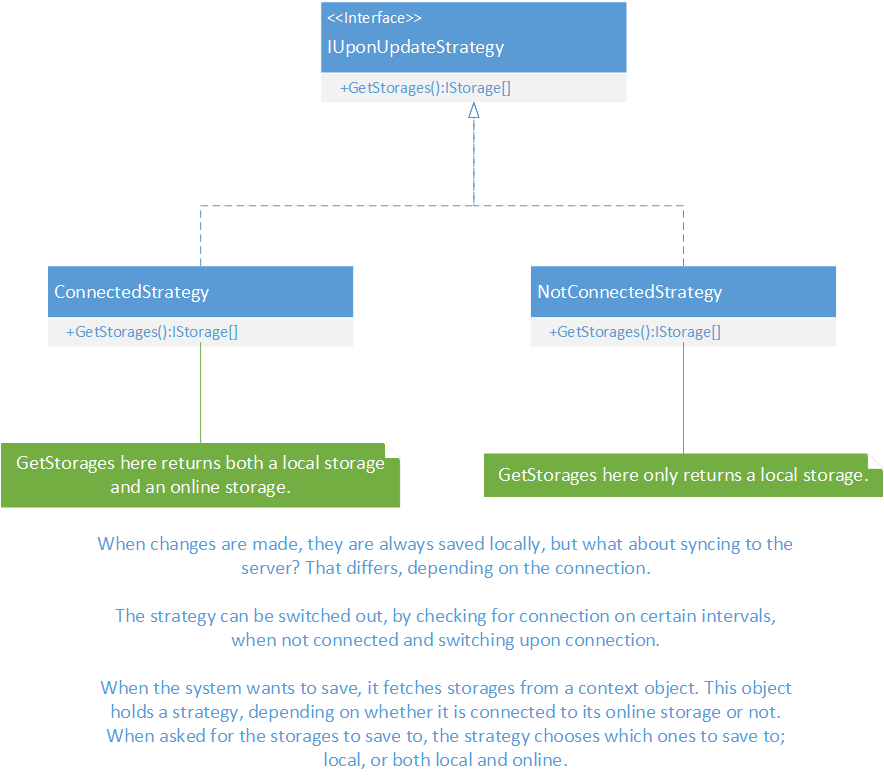
\includegraphics[scale=0.6]{figures/strategy_pattern.png}
\end{figure}

\begin{figure}[H]
  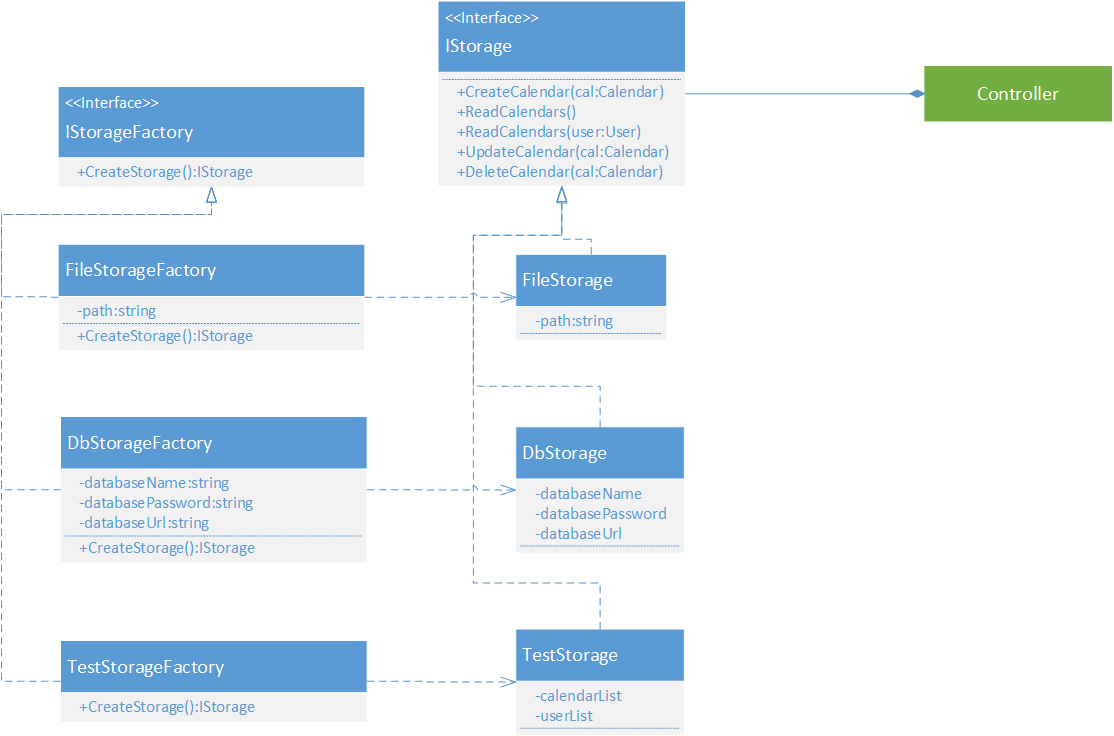
\includegraphics[scale=0.6]{figures/factory_pattern.png}
\end{figure}

\begin{figure}[H]
  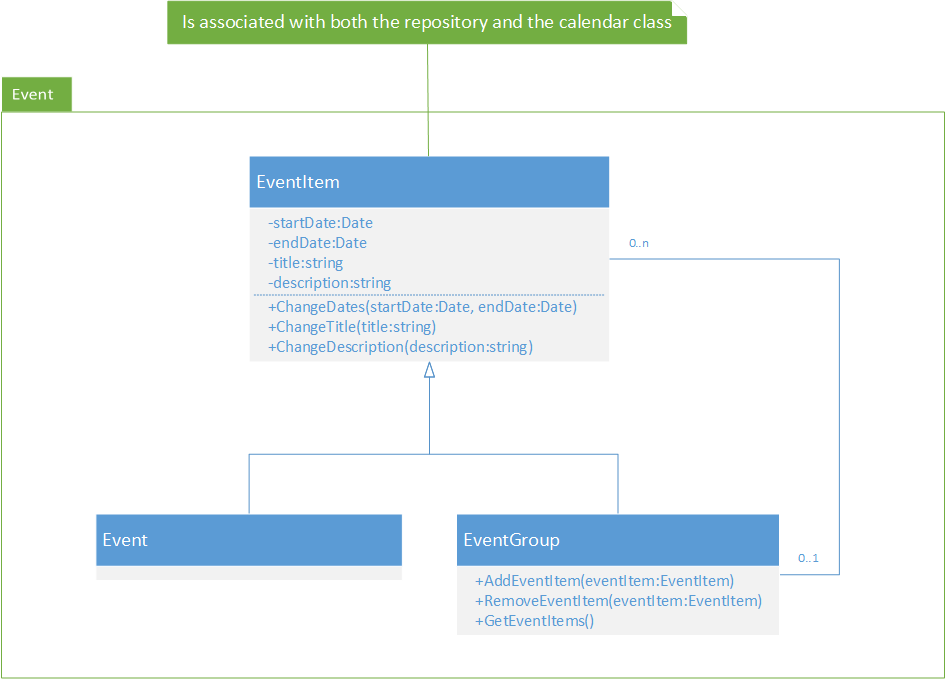
\includegraphics[scale=0.6]{figures/composite.png}
\end{figure}

\begin{figure}[H]
  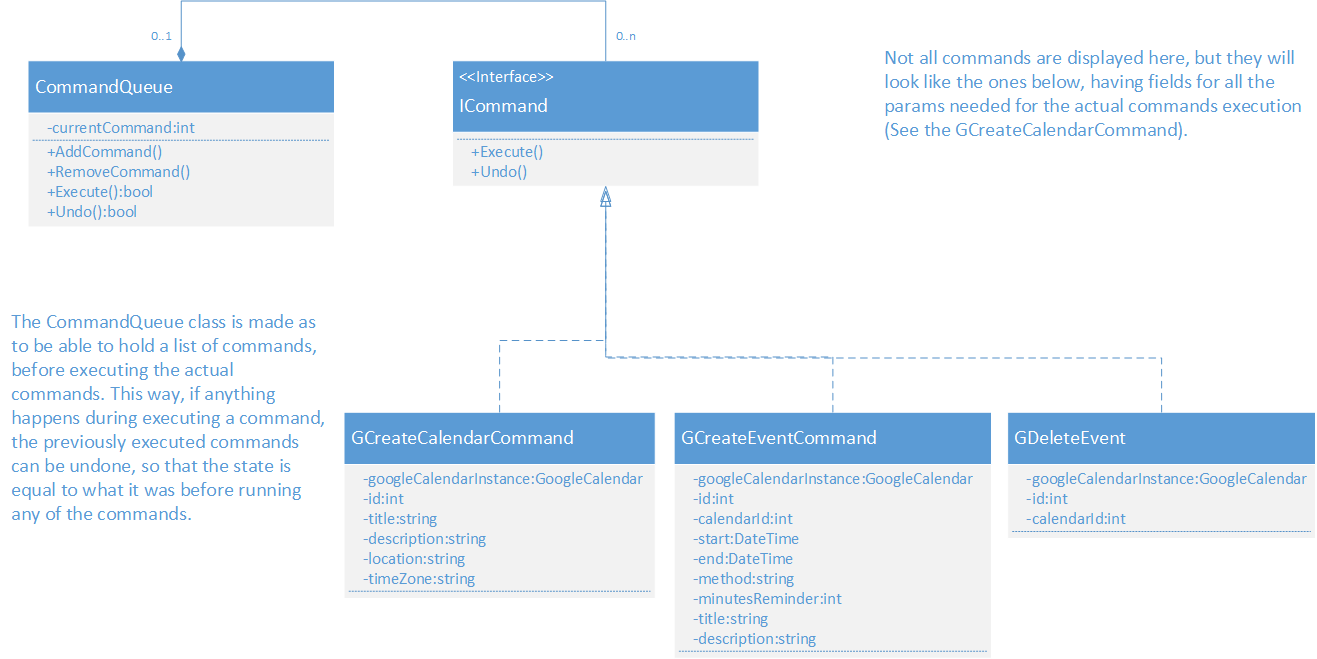
\includegraphics[scale=0.6]{figures/command.png}
\end{figure}

\subsection{Hardware/software mapping}
Two subsystems have been identified for this specific system implementation. A
system for the server, and a system for the client:\\
\textbf{ClientSubsystem}
\begin{itemize}
\item Calendar
\item Event
\item User
\item Date
\end{itemize}

\textbf{ServerSubsystem}
\begin{itemize}
\item Calendar
\item Event
\item User
\item Date
\end{itemize}

The following diagram shows the specific hardware relations between each
subsystem.
\begin{figure}[H]
  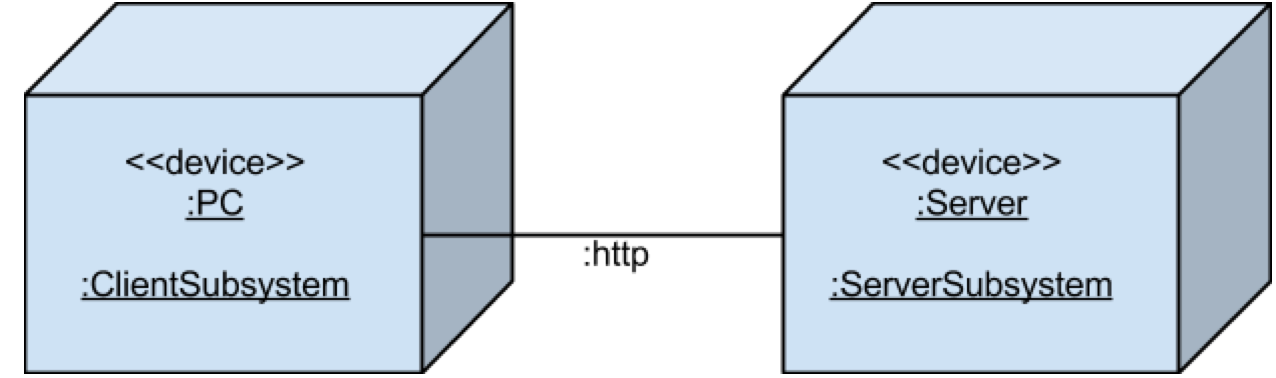
\includegraphics[scale=0.7]{figures/components.png}
\end{figure}

\subsection{Persistent data management}
The following data models have been considered suitable for persistent data
management:
\begin{itemize}
\item Calendars
\item Events
\item Users
\end{itemize}

\textbf{Calendars}  Need to be stored for access across multiple devices. This make
calendars persistent data. Events are what make up a calendar in its entirety,
so naturally these are also considered persistent data.


\textbf{Users} A users calendars are bound to the given user. The user data is required
to identify which calendars the user has access to.


Calendars are stored locally with all events, and synchronised to the
server. The calendars are stored in the iCalendar format (.ics, .ical,
etc). These calendar files are then synchronised to a file database on the
server.

\subsection{Access control and security}
Our access control is simple: once an unregistered user creates an account and
logs in, they are allowed to do everything except seeing other users private
events and calendars.

\begin{figure}[H]
  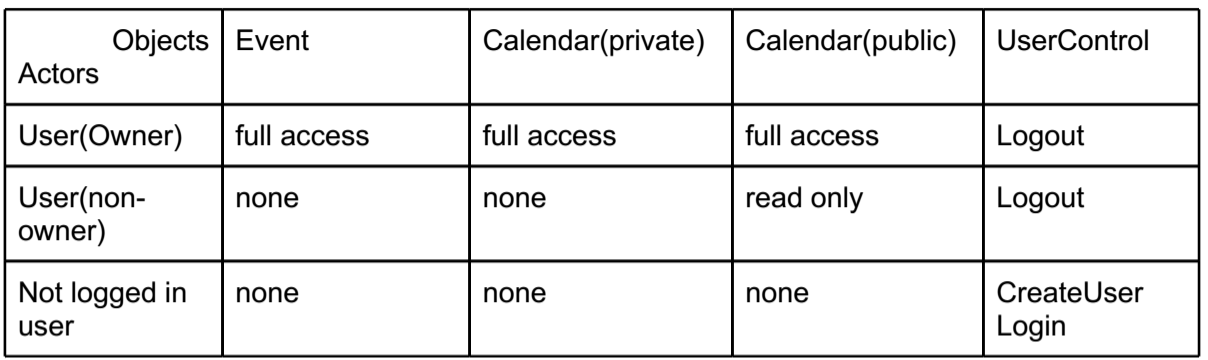
\includegraphics[scale=0.7]{figures/accesscontrol.png}
\end{figure}

\subsection{Global software control}
The global control flow is handled via the MVC architecture (event driven). This
means that there is a control that updates the view for the user, and the models
used by the system behind.

The views send the events to update the models. For instance if a user
clicks the add calendar button, an event is dispatched and the view shows the
add calendar form. If a user completes the action, an event is dispatched to
show the calendar view, and to the model to create the calendar. For error
handling/expanding the system, the model could send an event back to tell the
user whether the action succeeded or not.

\subsection{Boundary conditions}
An admin to start the service and shut it down.
The client is started by a user locally.
A user also exits the program.

The program should check up on data corruption through checksums on the files
synchronised. If the checksum is incomplete, or in any other way suspected to be
corrupted, then the last calendar with a valid checksum should be retrieved.

\section{Subsystem services}
\begin{center}
  \begin{figure}[H]
    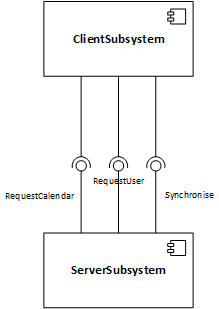
\includegraphics[scale=1.0]{figures/subsystemservices.png}
  \end{figure}
\end{center}

The server should present an interface for the client to use.  A client must be
able to fetch calendar and correct user data from the server, through these
interfaces. Furthermore there should be an interface for synchronisation.

%\section{Glossary}

\end{document}
